\documentclass{standalone}
\usepackage{tikz}
\usepackage{pgfplots}
\pgfplotsset{compat=newest}
\usepackage{pgfmath}
\usepackage{tikz-cd}
\usepackage{pgffor}
\usepackage{tkz-euclide}
\usetkzobj{all}
\usepgfplotslibrary{fillbetween}
\usetikzlibrary{
	calc,
	angles,
	quotes,
	arrows.meta,
	decorations.markings,
	math,
	backgrounds,
	pgfplots.statistics,
	matrix,
	patterns,
	shapes.geometric,
	spy,
	intersections,
}
\begin{document}
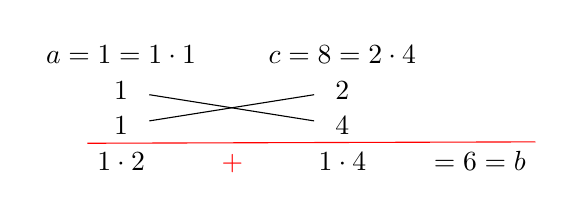
\begin{tikzpicture}
\matrix (m) [
                    matrix of math nodes,
                    row sep=-\pgflinewidth,
                    column sep=-.5\pgflinewidth,
                    minimum width=2em,
                ]
                { a=1=1\cdot1 & {} & c=8=2\cdot 4 &      \\
                    1           & {} & 2            &      \\
                    1           & {} & 4            &      \\
                    1\cdot 2    & {\color{red} +} & 1\cdot 4     & =6=b \\
                };
                \path
                (m-2-1) edge (m-3-3)
                (m-2-3) edge (m-3-1);
                \draw[red] (m-4-1.north west) -- (m-4-4.north east);
\end{tikzpicture}
\end{document}